\documentclass[11pt, a4paper]{article}
\usepackage{graphicx}
\usepackage{amsmath}
\usepackage{listings}
\usepackage{mathrsfs}



\title{Assignment 9} % Title

\author{Om Shri Prasath (EE17B113)} % Author name

\date{\today} % Date for the report
\begin{document}	

\maketitle % Insert the title, author and date
\section{Introduction}\label{introduction}

\begin{itemize}
  \item
    We explore digital fourier transform (DFT) with windowing. This is
    used to make the signal square integrable, and more specifically, that
    the function goes sufficiently rapidly towards 0 , also to make
    infinitely long signal to a finite signal, since to take DFT we need
    finite aperiodic signal.
  \item
    Windowing a simple waveform like \(cos(\omega t)\), causes its fourier
    transform to develop non-zero value at frequencies other than
    \(\omega\). This is called \emph{Spectral Leakage}. This can cause in
    some applications the stronger peak to smear the weaker contounter
    parts. So choosing proper windowing functions is essential. The
    windowing function we use is called \textbf{Hamming window} which is
    generally used in \(narrow-band\) \(applications\).
  \end{itemize}
 
\newpage
\section{Python Code}\label{code}

\subsection{Question 1:}\label{question-1}
\begin{itemize}
  \item
    Consider the function \(\cos^3(\omega_0 t)\). Obtain its spectrum for
    \(\omega_0 = 0.86\) with and without a Hamming window.
  \end{itemize}

\textit{\textbf{Code:}}
  \begin{lstlisting}
def f(t,n,w=None,d=None):
    if(n == 1):
        return sin(sqrt(2)*t)
    elif(n==2):
        if(w is None):
            return pow(cos(0.86*t),3)
        elif(w!=None):
            return pow(cos(w*t),3)
    elif(n==3):
        return cos(16*(1.5+t/(2*pi))*t)
    elif(n==4):
        return t
    elif(n==5):
        if(w is None):
            return cos(0.86*t)
        elif(w!=None and d!=None):
            return cos(w*t+d)
    else:
        return sin(sqrt(2)*t)   

def window_fn(n,N):
    return (0.54+0.46*cos(2*pi*n/N))

def findFFT(low_lim,up_lim,no_points,n,window=True,wo=None,d=None,eps=0):
    t = linspace(low_lim,up_lim,no_points+1)[:-1]
    dt=t[1]-t[0]
    fmax=1/dt
    N = no_points
    y = f(t,n,wo,d)+eps*randn(len(t))
    
    if(window):
        n1=arange(N)
        wnd=fftshift(window_fn(n1,N))
        y=y*wnd
        
    y[0]=0        
    y=fftshift(y) 
    Y=fftshift(fft(y))/N

    w = linspace(-pi*fmax,pi*fmax,N+1)[:-1]        
    return t,Y,w

def plot_FFT(t,Y,w,Xlims,plot_title,fig_no,dotted=False,Ylims=None):
    
    figure()
    subplot(2,1,1)
    
    if(dotted):
        plot(w,abs(Y),'b',w,abs(Y),'bo',lw=2)
    else:
        plot(w,abs(Y),'b',lw=2)

    xlim(Xlims)
        
    ylabel(r"$|Y(\omega)| \to$")
    title(plot_title)
    grid(True)
    
    ax = subplot(2,1,2)
    ii=where(abs(Y)>0.005)
    plot(w[ii],angle(Y[ii]),'go',lw=2)

    if(Ylims!=None):
        ylim(Ylims)
    
    xlim(Xlims)
    ylabel(r"$\angle Y(j\omega) \to$")
    xlabel(r"$\omega \to$")
    grid(True)
    savefig("fig10-"+fig_no+".png")
    show()

t,Y,w = findFFT(-4*pi,4*pi,256,2,True)
Xlims = [-8,8]
plot_title = r"Figure 8 : Spectrum of Windowed $\cos^3(\omega_o t)$"
plot_FFT(t,Y,w,Xlims,plot_title,"8")
t,Y,w = findFFT(-4*pi,4*pi,256,2,False)
Xlims = [-8,8]
plot_title = r"""Figure 9 : Spectrum of $\cos^3(\omega_o t)$ 
              without windowing"""
plot_FFT(t,Y,w,Xlims,plot_title,"9")
  \end{lstlisting}
  \newpage
  \begin{figure}[!tbh]
    \centering
    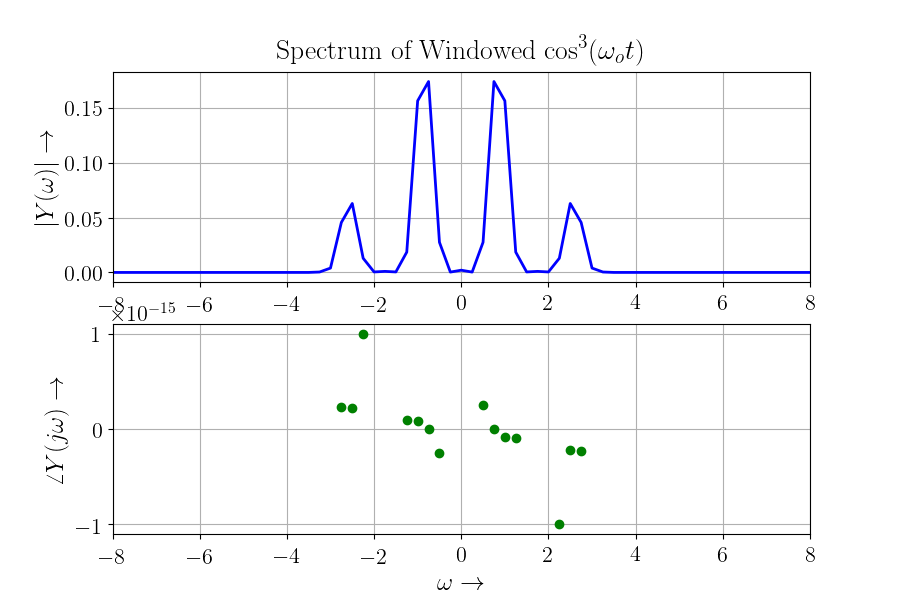
\includegraphics[scale=0.6]{./../Extras/fig10-8.png}  % Mention the image name within the curly braces. Image should be in the same folder as the tex file.  
    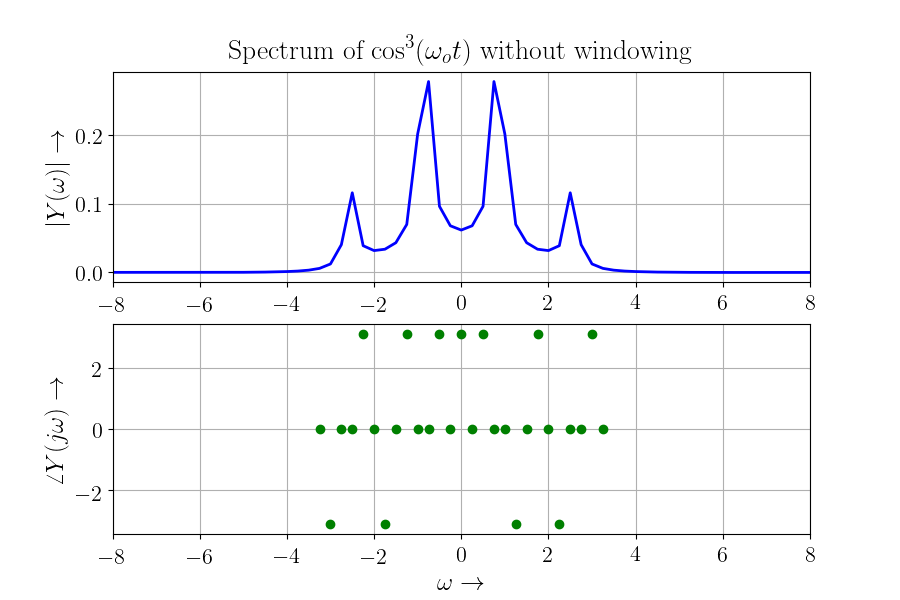
\includegraphics[scale=0.6]{./../Extras/fig10-9.png}  % Mention the image name within the curly braces. Image should be in the same folder as the tex file.  
    \caption{Spectrum of $\cos^3(\omega_o t)$ with and without windowing}
  \end{figure}
  \newpage
  \subsubsection{Results and Discussion:}\label{results-and-discussion}

  \begin{itemize}
  \item
    Here we can see clear differences between the windowed fourier
    transform and fourier transform without application of windows. Peak
    is being smeared by the windowing function but the stary high
    frequency components are attenuated by the window function. The
    \emph{spectral leakage} can also be noticed.
  \end{itemize}
  \newpage
  \subsection{Question 2:}\label{question-3}

  \begin{itemize}
  
  \item
    Write a program that will take a 128 element vector known to contain
    \(\cos(\omega_0 t + \delta)\) for arbitrary \(\delta\) and
    \(0.5 < \omega_0 < 1.5\) where \(\pi \leq t \leq \pi\).
  \item
    You have to extract the digital spectrum of the signal, find the two
    peaks at \(\pm \omega_0\), and estimate \(\omega_0\) and \(\delta\).
  \end{itemize}
  
   \subsubsection{Estimating \(\omega\) and \(\delta\) from fourier spectrum}
  
  \begin{itemize}
  \item
    According to the question the if the spectra is obtained, the
    resolution is not enough to obtain the \(\omega_0\) directly. The peak
    will not be visible clearly because of the fact that resolution of the
    frequecny axis is not enough. So a statistic is necessary to estimate
    value of \(\omega_0\)
  \item
    Let,
  \end{itemize}
  
  \begin{equation}
  \mu = Mean(|Y(\omega)|)
  \end{equation}
  
  \begin{equation}
  \sigma = Standard\ Deviation(|Y(\omega)|)
  \end{equation}
  
  \begin{equation}
  \omega_0 = \frac{\sum \omega_i |Y(\omega_i)|}{\sum |Y(\omega_i)|} \\
  \\
  \forall \omega_i\ where\ |Y(\omega_i)| > \mu + 0.1\sigma
  \end{equation}
  
  \begin{itemize}
  \item
    Which is essentially the weighted average of \(\omega\) where weights
    are \(|Y(\omega)|\) subject to constraint that \(|Y(j\omega)|\) must
    be greater than a value as specified in the formula.
  \item
    Now, \(\delta\) can be found by two ways :
  \item
    Least square fitting of
  \end{itemize}
  
  \begin{equation}
  y(t) = A\cos(\omega_0 t) + B\sin(\omega_0 t)
  \end{equation}
  
  \begin{itemize}
  
  \item
    Minimizing L2-norm to find the coefficients \(A, B\), we can compute
    \(\delta\) by,
  \end{itemize}
  
  \begin{equation}
  \delta = -\tan^{-1}(\frac{B}{A})
  \end{equation}
  
  \begin{itemize}
  \item
    Another method which can be used is to find the phase of the discrete fourier transform at \(\omega_o\)
    nearest to estimated \(\omega\) using the above statistic.
  \item
    This works because the phase of \(\cos(\omega_o t+\delta)\) when
    \(\delta = 0\) is 0, so when its not its \(\delta\), so we can
    estimate it by this approach.
  \item
    The latter approach is used in this assignment.
  \end{itemize}
  
\textit{\textbf{Code:}}
  \begin{lstlisting}
def estimate_omega(low_lim,up_lim,eps):
    w_actual = np.random.uniform(low_lim,up_lim)
    delta_actual = (randn())
    t,Y,w = findFFT(-1*pi,1*pi,128,5,True,w_actual,delta_actual,eps=eps)
    
    Y_half = Y[int(len(Y)/2):]
    w_half = w[int(len(w)/2):]
    k = 0.1
    idx = 
    np.where(abs(Y_half) >= np.mean(abs(Y_half))+
                                  k*sqrt(np.var(abs(Y_half))))
    
    w0 = np.matmul(w_half[idx],
                   np.transpose(abs(Y_half[idx])))/
                                            (np.sum(abs(Y_half[idx])))
    
    w_peak_idx = (np.abs(w_half-w0)).argmin()
    delta      = angle(Y_half[w_peak_idx])
    
    print("Actual w0 : %g , Actual delta : %g"%(w_actual,delta_actual))



    return t,w0,delta,w_actual,delta_actual


def createAmatrix(nrow,t,model,wo):
    A = zeros((nrow,2)) 
    A[:,0],A[:,1] = model(t,wo)
    return A

def modelA(t,wo):
    return (cos(wo*t),sin(wo*t))
def estimate_delta(t,wo,y):
    M = createAmatrix(len(y),t,modelA,wo)
    c = (lstsq(M,y)[0])
    
    delta = arccos(c[0]/sqrt(pow(c[0],2)+pow(c[1],2)))
    return delta
def estimator(N,eps):
    est_err_w = []
    est_err_delta = []
    for i in range(N):
        t,wo_est,delta_est,w_actual,delta_actual = 
                          estimate_omega(0.5,1.5,eps)


        est_err_w.append(abs(amax(w_actual-wo_est)))
        est_err_delta.append(abs(amax(delta_actual-delta_est)))
        
        print("Estimated w0 : %g and delta : %g \n"%((wo_est),delta_est))
    return np.mean(est_err_w),np.mean(est_err_delta)

eps = 0
N = 5

estimated_error_w,estimated_error_delta = estimator(N,eps)

print("\nEstimated Error for %g sample signals without Noise addition 
in w0 and delta : %g , %g"%(N,estimated_error_w,estimated_error_delta))


  \end{lstlisting}
  \subsubsection{Results and Discussion:}\label{results-and-discussion}

\begin{itemize}
\item


Estimated Error for 5 sample signals without Noise addition in w0 and delta : 0.117576 , 0.0214041

\item
  As we observe that actual \(\omega\) \& \(\delta\) are generated using
  uniformly distributed random functions, and using the above center of
  mass statistic we get estimated ones close with error in order of 1\%
\end{itemize}
		\newpage
\subsection{Question 3:}\label{question-4}

\begin{itemize}

\item
  Now we add \textbf{white gaussian noise} to data in \(Q_3\). This can
  be generated by \(randn()\) in python. The extent of this noise is
  \(0.1\) in amplitude (i.e., \(0.1*randn(N)\), where \(N\) is the
  number of samples).
\item
  Repeat the problem and find the \(\omega_0\) and \(\delta\)
\end{itemize}

\textit{\textbf{Code:}}
\begin{lstlisting}
  eps = 0.1
  N   = 5
  
  estimated_error_w,estimated_error_delta = estimator(N,eps)
  
  print("\nEstimated Error for %g sample signals with Noise addition in 
  w0 and delta : %g , %g"% (N,estimated_error_w,estimated_error_delta))
      
\end{lstlisting}
\subsubsection{Results and Discussion:}\label{results-and-discussion}

\begin{itemize}
\item
Estimated Error for 5 sample signals with Noise addition in w0 and delta : 0.12154 , 0.0247817

\item
  Now we have added noise to the function and tried to estimate \(\omega\) \&
  \(\delta\) from the spectrum.
\item
  We follow same procedure as above case and we can observe that
  \(\omega\) \& \(\delta\) are generated using uniformly distributed
  random functions, and using the above center of mass statistic we get
  estimated ones close with error in order of 10\% in \(\omega\) and 1\%
  in \(\delta\)
\item
  This error is slightly higher compared to the case without noise as we
  expected.
\end{itemize}
\newpage
\subsection{Question 4 - Analysis of Chirped Signal
Spectrum}\label{question-5---analysis-of-chirped-signal-spectrum}

\begin{itemize}

\item
  Plot the \(DFT\) of the function
  \(\cos(16 \ (1.5 + \frac{t}{2\pi}) \ t)\) where
  \(-\pi \leq t \leq \pi\) in \(1024\) steps. This is known as a
  \(chirped\) signal.
\item
  Its frequency continuously changes from \(16\) to \(32\) radians per
  second. This also means that the period is \(64\) samples near
  \(−\pi\) and is \(32\) samples near \(+\pi\).
\end{itemize}

\textit{\textbf{Code:}}
\begin{lstlisting}
def chirp(t):
    return cos(16*(1.5+t/(2*pi))*t)
t = linspace(-pi,pi,1025)[:-1]
dt=t[1]-t[0]
fmax=1/dt
N = 1024
y = chirp(t)
Y=fftshift(fft(y))/N
w = linspace(-pi*fmax,pi*fmax,N+1)[:-1]       
Xlims = [-100,100]
plot_title = r"Spectrum of Non-Windowed Chirped Signal"
plot_FFT(t,Y,w,Xlims,plot_title,"10")
t = linspace(-pi,pi,1025)[:-1]
dt=t[1]-t[0]
fmax=1/dt
N = 1024
y = chirp(t)

n1=arange(N)
wnd=fftshift(window_fn(n1,N))
y=y*wnd
y[0] = 0
y = fftshift(y)
Y = fftshift(fft(y))/1024.0
w = linspace(-pi*fmax,pi*fmax,1025)[:-1]       

Xlims = [-100,100]
plot_title = r"Spectrum of Windowed Chirped Signal"
plot_FFT(t,Y,w,Xlims,plot_title,"11")

\end{lstlisting}
\newpage
\begin{figure}[!tbh]
  \centering
  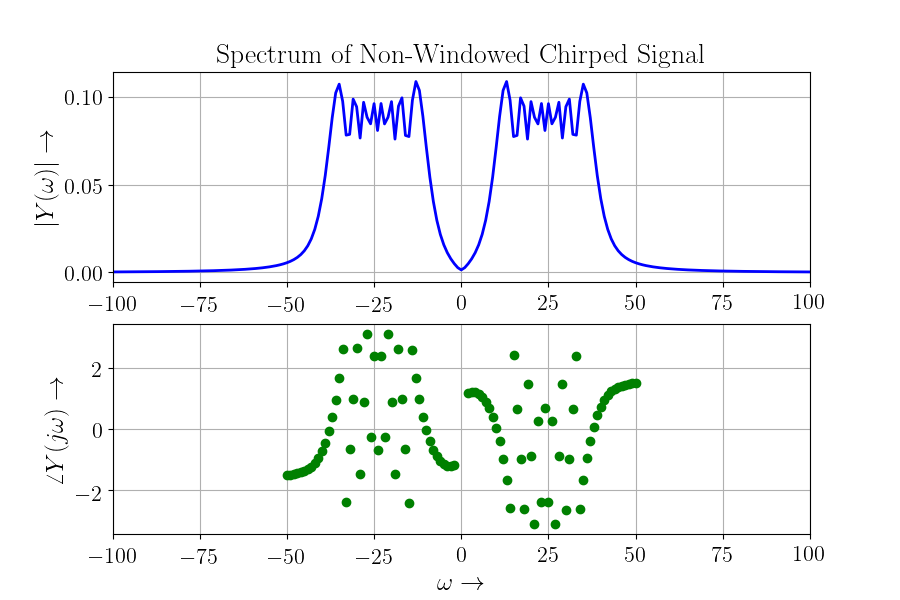
\includegraphics[scale=0.6]{./../Extras/fig10-10.png}  % Mention the image name within the curly braces. Image should be in the same folder as the tex file.  
  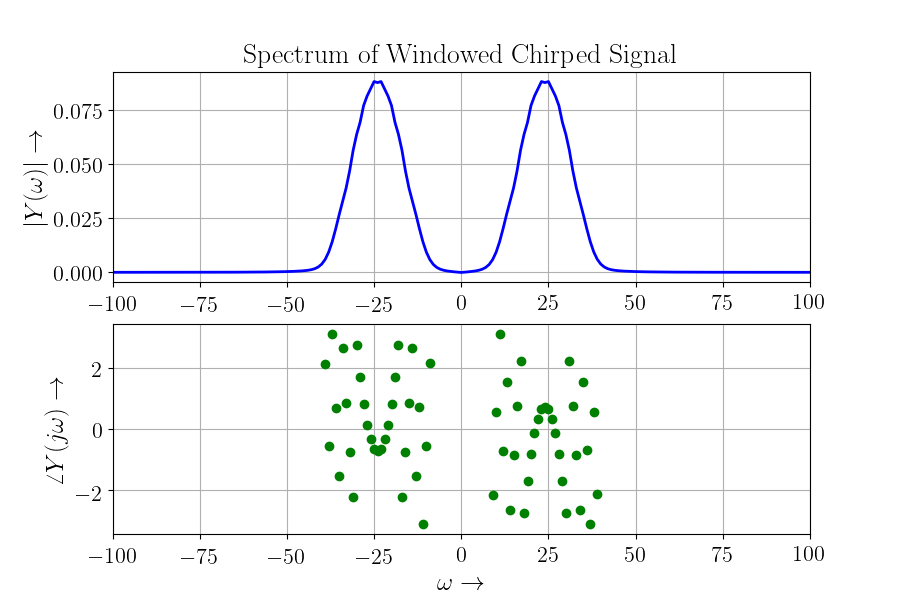
\includegraphics[scale=0.6]{./../Extras/fig10-11.png}  % Mention the image name within the curly braces. Image should be in the same folder as the tex file.  
  \caption{Spectrum of chirped signal with and without windowing}
\end{figure}
\newpage
\subsection{Question 5:}\label{question-6}

\begin{itemize}

\item
  For the same chirped signal, break the \(1024\) vector into pieces
  that are \(64\) samples wide. Extract the \(DFT\) of each and store as
  a column in a 2D array.
\item
  Then plot the array as a surface plot to show how the frequency of the
  signal varies with time.
\item
  Plot and analyse the \textbf{time frequency} plot, where we get
  localized \(DFTs\) and show how the spectrum evolves in time.
\item 
We are going to implement this using \textbf{Short time Fourier Transform} (STFT)  
\item
  From the 1024 dimensional vector, we take 64 dimensional sub-vector,
  and find the fourier transform and we will see how it evolves in
  time.This is known as \textbf{Short time Fourier Transform} (STFT)
\end{itemize}

\textit{\textbf{Code:}}
\begin{lstlisting}
def partition(t,n):
  t_batches = [t[i:n+i] for i in range(len(t)-n)]
  return t_batches
def STFT(t,no_samples,n):
  dt=t[1]-t[0]

  fmax=1/dt
  N = no_samples
  y = f(t,n)
  
  n1=arange(N)
  wnd=fftshift(window_fn(n1,N))
  y=y*wnd
      
  Y=fftshift(fft(y))/N
  
  w = linspace(-pi*fmax,pi*fmax,N+1)[:-1]        
  return t,Y,w
n = 64
t_batches = partition(t,n)

batch_dfts = []
batch_ts   = []

for i in range(len(t_batches)):
  t,Y,w = STFT(t_batches[i],n,3)
  batch_dfts.append(Y)
  batch_ts.append(t)
t = linspace(-pi,pi,1025)[:-1]
T, W = np.meshgrid(t[:960],w)
Z = abs(np.array(batch_dfts))
fig = figure()
ax = fig.add_subplot(111)
ax.contourf(T,W,Z.T,cmap='jet')
title("Contour plot of the magnitude of the spectrum")
xlabel(r"$time \to$")
ylabel(r"$\omega \to$")
plt.savefig("fig10-12.png")
show()
fig = plt.figure()
ax = fig.gca(projection='3d')

surf = ax.plot_surface(T,W,(Z.T), cmap=cm.jet,
                     linewidth=0.1)

title(r"Surface plot of $|Y(\omega)|$")
ax.set_xlabel(r'$t \to$')
ax.set_ylabel(r'$\omega \to$')
ax.set_zlabel(r'$|Y(\omega)| \to$')


fig.colorbar(surf, shrink=0.5, aspect=5)
plt.savefig("fig10-13.png")
plt.show()
\end{lstlisting}
\newpage
\begin{figure}[!tbh]
  \centering
  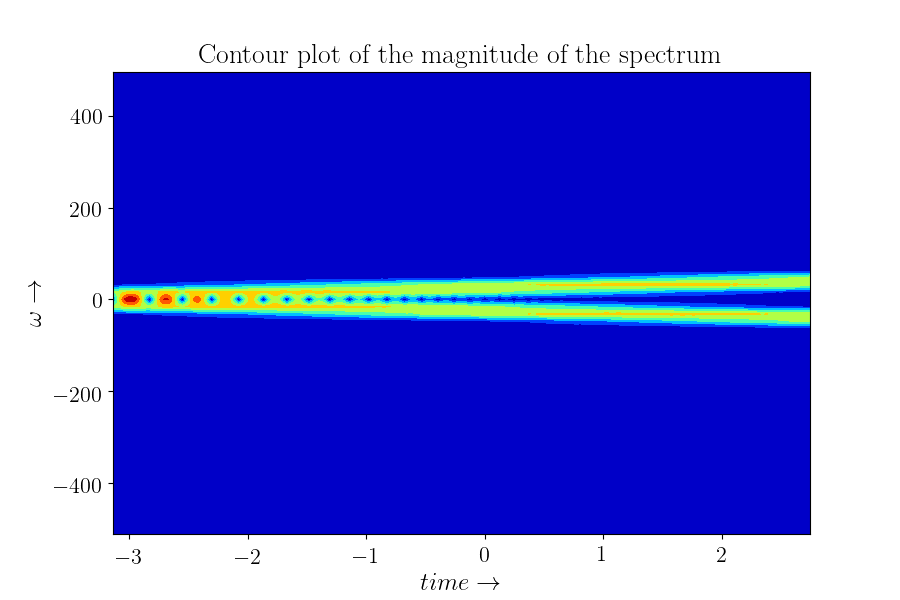
\includegraphics[scale=0.6]{./../Extras/fig10-12.png}  % Mention the image name within the curly braces. Image should be in the same folder as the tex file.  
  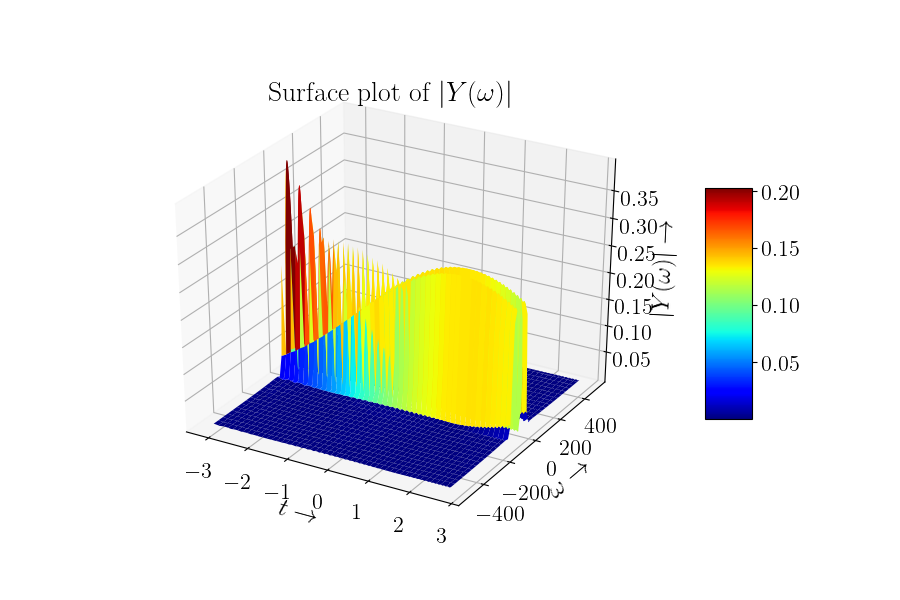
\includegraphics[scale=0.6]{./../Extras/fig10-13.png}  % Mention the image name within the curly braces. Image should be in the same folder as the tex file.  
  \caption{Contour plot and Surface plot of the magnitude of broken chirped signal}
\end{figure}
\newpage
\subsubsection{Results \& Discussion:}\label{results-discussion}

\begin{itemize}
  \item
  We observe that the magnitude of the fourier transform splits as time
  progresses as the frequency of the signal increases.
\item
  In the surface plot of magnitude of spectrum vs time vs frequency, we observe strong peaks and as inferred from the contour plot of
  the magnitude spectrum we see 2 lobes whose separation increases as
  time increases.
\end{itemize}

	

	
		
    \section{Conclusion :}\label{conclusion}

\begin{itemize}

\item
  Here in this assignment we implemented windowed fourier transform and
  also understood the need for windowing and also effects of windowing.
\item
  Moreover,we implemented \textbf{Short time Fourier Transform} and
  witnessed how fourier transform evolves in time.
\end{itemize}

	

\end{document}